\section{Technician license test overview}
\frame{\mysectionpage}

{
    \usebackgroundtemplate{%
      \vbox to \paperheight{\vfil\hbox to \paperwidth{\hfil
\includegraphics[height=\paperheight]{img/simpsons/skinner-test.jpg}\hfil}\vfil}
    }
    \frame{}
}

\begin{frame}
    \only<1>{
\includegraphics[width=0.9\textwidth]{img/simpsons/rules.png} \\}
    \only<2>{
\includegraphics[width=0.9\textwidth]{img/simpsons/procedures.png} \\}
    \only<3>{
\includegraphics[width=0.9\textwidth]{img/simpsons/homer-simpson-decisions.jpg} \\}
    \only<4>{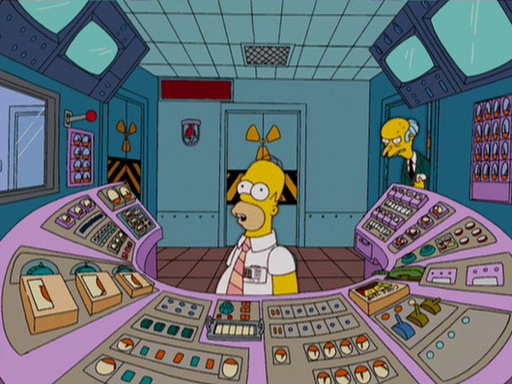
\includegraphics[width=0.9\textwidth]{img/simpsons/homer-workspace.png} \\}
\end{frame}

\begin{frame}[t]{Sections of the Technician test}
    \begin{columns}[onlytextwidth]
        \column{0.5\textwidth}
            \begin{enumerate}
                \item[T1] \hilitem<1>{FCC Rules, Operator responsibilities}
                \item[T2] \hilitem<2>{Operating procedures}
                \item[T3] \hilitem<3>{Radio wave characteristics and propagation}
                \item[T4] \hilitem<4>{Equipment practices, station setup}
            \end{enumerate}
        \column{0.5\textwidth}
            \centering
%            \only<1>{%
%                
\includegraphics[width=0.9\textwidth]{img/simpsons/rules.png} \\
%                Various amateur services, administrative vocabulary, international transmission, handling call signs
%            }
%            \only<2>{%
%                
\includegraphics[width=0.9\textwidth]{img/simpsons/procedures.png} \\
%                Choosing a frequency, calling another station, testing transmissions, CTCSS, squelch, CW vs. AM vs. SSB vs. FM, emergency traffic
%            }
%            \only<3>{
%                
\includegraphics[width=0.9\textwidth]{img/simpsons/homer-simpson-decisions.jpg} \\
%                Choosing a frequency, calling another station, testing transmissions, CTCSS, squelch, CW vs. AM vs. SSB vs. FM, emergency traffic
%            }
%            \only<4>{%
%                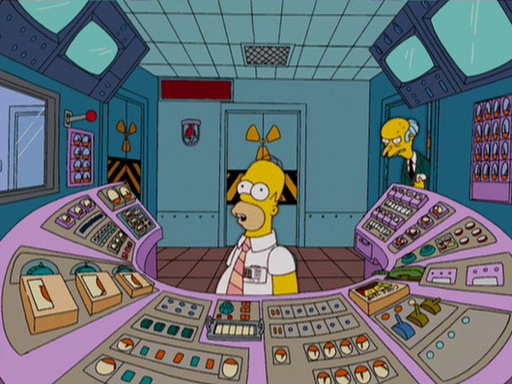
\includegraphics[width=0.9\textwidth]{img/simpsons/homer-workspace.png} \\
%                Microphones, speakers, power supplies, filters, computers, RF grounding, tuning, repeater offset
%            }

%SUBELEMENT T4 - Amateur radio practices and station setup � [2 Exam Questions - 2 Groups]
%
%T4A � Station setup; microphone, speaker, headphones, filters, power source, connecting a computer, RF grounding
%
%T4B - Operating controls; tuning, use of filters, squelch, AGC, repeater offset, memory channels
%
%
%SUBELEMENT T5 � Electrical principles, math for electronics, electronic principles, Ohm�s Law � [4 Exam Questions - 4 Groups]
%
%T5A - Electrical principles; current and voltage, conductors and insulators, alternating and direct current
%
%T5B - Math for electronics; decibels, electronic units and the metric system
%
%T5C - Electronic principles; capacitance, inductance, current flow in circuits, alternating current, definition of RF, power calculations
%
%T5D � Ohm�s Law
%
%
%SUBELEMENT T6 � Electrical components, semiconductors, circuit diagrams, component functions � [4 Exam Groups - 4 Questions]
%
%T6A - Electrical components; fixed and variable resistors, capacitors, and inductors; fuses, switches, batteries
%
%T6B � Semiconductors; basic principles of diodes and transistors
%
%T6C - Circuit diagrams; schematic symbols
%
%T6D - Component functions
%
%
%SUBELEMENT T7 � Station equipment, common transmitter and receiver problems, antenna measurements and troubleshooting, basic repair and testing � [4 Exam Questions - 4 Groups]
%
%T7A - Station radios; receivers, transmitters, transceivers
%
%T7B � Common transmitter and receiver problems; symptoms of overload and overdrive, distortion, interference, over and under modulation, RF feedback, off frequency signals; fading and noise; problems with digital communications interfaces
%
%T7C � Antenna measurements and troubleshooting; measuring SWR, dummy loads, feedline failure modes
%
%T7D � Basic repair and testing; soldering, use of a voltmeter, ammeter, and ohmmeter
%
%
%
%SUBELEMENT T8 � Modulation modes, amateur satellite operation, operating activities, non-voice communications � [4 Exam Questions - 4 Groups]
%
%T8A � Modulation modes; bandwidth of various signals
%
%T8B - Amateur satellite operation; Doppler shift, basic orbits, operating protocols
%
%T8C � Operating activities; radio direction finding, radio control, contests, special event stations, basic linking over Internet
%
%T8D � Non-voice communications; image data, digital modes, CW, packet, PSK31
%
%
%SUBELEMENT T9 � Antennas, feedlines [2 Exam Groups - 2 Questions]
%
%T9A � Antennas; vertical and horizontal, concept of gain, common portable and mobile antennas, relationships between antenna length and frequency
%
%T9B - Feedlines; types, losses vs. frequency, SWR concepts, matching, weather protection, connectors
%
%
%SUBELEMENT T0 � AC power circuits, antenna installation, RF hazards � [3 Exam Questions - 3 Groups]
%
%T0A � AC power circuits; hazardous voltages, fuses and circuit breakers, grounding, lightning protection, battery safety, electrical code compliance
%
%T0B � Antenna installation; tower safety, overhead power lines
%
%T0C - RF hazards; radiation exposure, proximity to antennas, recognized safe power levels, exposure to others

    \end{columns}
\end{frame}

%SUBELEMENT T1 � FCC Rules, descriptions and definitions for the amateur radio service, operator and station license responsibilities - [6 Exam Questions - 6 Groups]
%
%T1A - Amateur Radio services; purpose of the amateur service, amateur-satellite service, operator/primary station license grant, where FCC rules are codified, basis and purpose of FCC rules, meanings of basic terms used in FCC rules
%
%T1B - Authorized frequencies; frequency allocations, ITU regions, emission type, restricted sub-bands, spectrum sharing, transmissions near band edges
%
%T1C - Operator classes and station call signs; operator classes, sequential, special event, and vanity call sign systems, international communications, reciprocal operation, station license licensee, places where the amateur service is regulated by the FCC, name and address on ULS, license term, renewal, grace period
%
%T1D - Authorized and prohibited transmissions
%
%T1E - Control operator and control types; control operator required, eligibility, designation of control operator, privileges and duties, control point, local, automatic and remote control, location of control operator 
%
%T1F - Station identification and operation standards; special operations for repeaters and auxiliary stations, third party communications, club stations, station security, FCC inspection
%
%
%SUBELEMENT T2 - Operating Procedures - [3 Exam Questions - 3 Groups]
%
%T2A - Station operation; choosing an operating frequency, calling another station, test transmissions, use of minimum power, frequency use, band plans
%
%T2B � VHF/UHF operating practices; SSB phone, FM repeater, simplex, frequency offsets, splits and shifts, CTCSS, DTMF, tone squelch, carrier squelch, phonetics
%
%T2C �Public service; emergency and non-emergency operations, message traffic handling
%
%
%SUBELEMENT T3 � Radio wave characteristics, radio and electromagnetic properties, propagation modes � [3 Exam Questions - 3 Groups]
%
%T3A - Radio wave characteristics; how a radio signal travels; distinctions of HF, VHF and UHF; fading, multipath; wavelength vs. penetration; antenna orientation
%
%T3B - Radio and electromagnetic wave properties; the electromagnetic spectrum, wavelength vs. frequency, velocity of electromagnetic waves 
%
%T3C - Propagation modes; line of sight, sporadic E, meteor, aurora scatter, tropospheric ducting, F layer skip, radio horizon
%
%
